\chapter{Experiment and Evaluation}
\graphicspath{{Chapter5/Figs/}}

\begin{chapabstract}
Firstly, we introduce the dataset used for training and evaluating in our experiments. We also present the evaluation metrics and explain the reason for choosing those criteria. Then, the experiment results are shown in comparing to other proposed models. Finally, we present how to set up the environments for experiments.
\end{chapabstract}

\section{Dataset}
\label{sec:dataset}

We tried to collect and use data from various sources, i.e., VirusTotal VirusBay, VirusShare, Malware DB, and Microsoft Malware Classification Challenge. But there are many issues which those datasets. The amount of malicious files is much more massive than the number of benign files because almost benign binaries are often protected by copyright laws. Further, malware analysis and data labeling are consuming processes and required well-trained security engineers. Additionally, there are many risks in publishing a large dataset that includes malicious binaries. Therefore, it is hard to find an ideal dataset.

Fortunately, in April 2018, Endgame, Inc (a computer security company from Virginia, United States) published EMBER dataset, a labeled benchmark dataset for training machine learning-based static PE file malware detector \cite{anderson2018ember}. The dataset includes features extracted from 1.1M binary files: 900K training samples (300K malicious, 300K benign, 300K unlabeled) and 200K test samples (100K malicious, 100K benign).

\begin{figure}[H] 
\centering
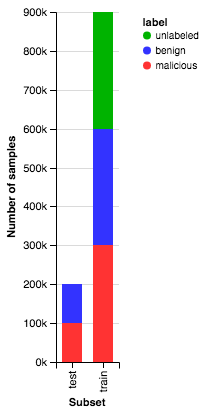
\includegraphics[height=0.4\textheight]{data_subset.png}
\caption{Distribution of samples in the dataset \cite{anderson2018ember}.}
\label{fig:ember}
\end{figure}
 
The EMBER dataset is the sizeable public dataset for malware detection which must include benign files and have an ideal ratio of malicious and benign files for machine learning tasks. This will solve the common problem of predictive accuracy, i.e., it will be misleading when the data is imbalanced. For example, if 99\% of your data is benign, then just blindly labeling everything as benign will achieve 99\% accuracy.

We decided to use 600,000 labeled training samples and all the test samples in evaluating our models.

\section{Evaluation Criteria}

As discussed in section \ref{sec:objectives}, the goal of the thesis is to find a machine learning-based malware detection method that operates at a meager false positive rate while tries to achieve a high detection rate.

\subsection{False Alarm Rate}

False positives, or false alarms, happen when a detector mistakes a malicious label for a benign file. We intend to make the false positive rate as low as possible, which is untypical for machine learning application. It is important because even one false alarm in a thousand benign files can create severe consequences for users. For examples, a report published in 2015 shows that many organizations in the United States consumed massive amounts of money on dealing with inaccurate malware warnings \cite{eduard2015false}. Moreover, according to a survey of IT administrators in 2017 \cite{jonathan2017survey}, 42 percent of companies consider that their users lost productivity as an effect of false-alarm results, which creates a choke point for IT administrators in the business life cycle. This problem is complicated by the fact that there are lots of clean files in the world, they keep appearing, and it is more challenging to collect these files. 

\begin{center}
    ${False\ alarm\ rate} =  \frac{\sum False\ positive}{\sum Condition\ negative}$
\end{center}

We evaluate the accuracy of our approaches at two specific false alarm rate values: at less than 0.1\%, and at less than 1\%.

\subsection{Detection Rate}

The detection rate, (eqv. with recall or true positive rate), measures the ratio of malicious programs detected out of the malware files used for testing. With higher recall, fewer actual cases of malware go undetected.

\begin{center}
    ${Detection\ rate} =  \frac{\sum True\ positive}{\sum Condition\ positive}$
\end{center}

In reality, the true positive rate shows the potential of how unseen binaries that were detected.

\subsection{AUROC}

As introduced in section \ref{ssec:auroc}, AUROC, or AUC, stands for \textit{Area under the ROC Curve} and provides an aggregate measure of performance across all possible classification thresholds.

AUC is scale-invariant and measures how well predictions are ranked, rather than their absolute values. Besides, AUC is classification-threshold-invariant, so that it can measure the quality of the predictions irrespective of what threshold is chosen.

A rough guide for classifying the accuracy of a classification test is the typical academic point system: 

\begin{itemize}
\item 0.9 - 1.0 = Excellent
\item 0.8 - 0.9 = Good
\item 0.7 - 0.8 = Fair
\item 0.6 - 0.7 = Poor
\item 0.5 - 0.6 = Fail
\end{itemize}

\section{Experimental Results}

The inputs of the model are vectors of dimension 1711, which are achieved after pre-processing as described in section \ref{sec:feature-extraction}. From the vectorized data, we trained a gradient boosting decision tree model using LightGBM framework \cite{ke2017lightgbm}. 

All our experiments were run on an instance in Google Cloud platform, which has 24 vCPUs and 32 GB memory (section \ref{sec:research-env} shows how to set up the research environment). With using parallel programming, it took about 10 minutes to vectorize the raw features and about 5 minutes to train the model. 

As mention in section \ref{sec:dataset}, we evaluated our system with 200,000 samples, which has 1:1 ratio of malicious and clean files. The ROC curve of the final model is shown in Figure \ref{fig:roc_curve_with_highlights}, and the distribution of scores for testing samples is shown in Figure \ref{fig:score_dist}.

\begin{figure}[h]
\centering
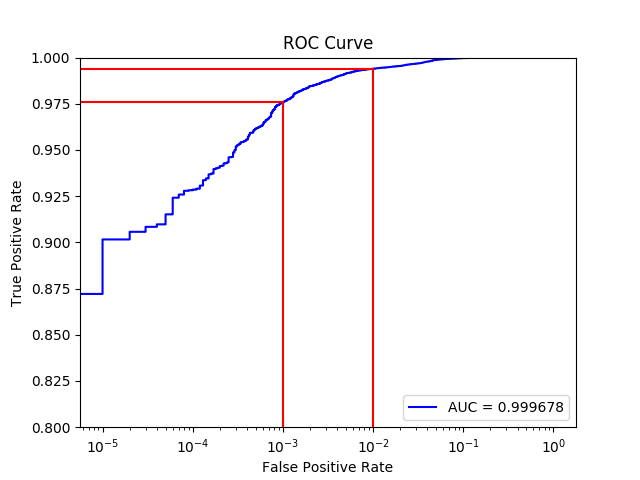
\includegraphics[width=\textwidth]{roc_curve_with_highlights.png}
\caption{The ROC curve of proposed model}
\label{fig:roc_curve_with_highlights}
\end{figure}

\begin{figure}[h] 
\centering
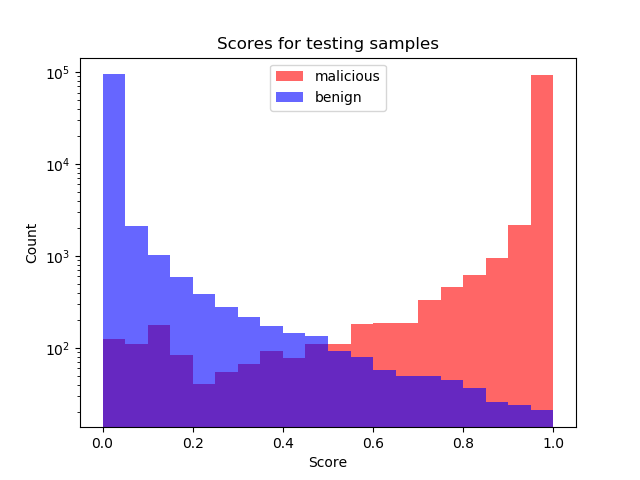
\includegraphics[width=\textwidth]{score_dist.png}
\caption{The distribution of scores for testing samples}
\label{fig:score_dist}
\end{figure}

The area under ROC curve exceeds $0.999661$ with the threshold, and with a threshold of $0.828987$, the model score results in less than $0.1\%$ false alarm rate at a detection rate $97.5720\%$. At less than $1\%$ false positive rate, the model exceeds $99.3940\%$ detection rate with a threshold of $0.307897$. 

The baseline model, provided by the dataset publishers \cite{anderson2018ember}, has the Area under the ROC curve of $0.999678$, score results in less than $0.1\%$ FPR at TPR exceeding $92.99\%$, and at less than $1\%$ FPR, it exceeds $98.2\%$ TPR. In comparing, our model has better performance because of hyper-parameter tuning, and it also takes less time for training as a result of reducing feature space. 

\section{Environment Setup Guide} 
\label{sec:research-env}

We mainly use the cross-platform tools in research and development for easily switching between operating systems. We use a Windows 10 Pro virtual machine for static malware analysis, an Ubuntu 16.04 LTS cloud instance for training and testing machine learning models, and use PyCharm Professional as mainly Integrated development environment (IDE).

\subsection{Windows environment for static analysis}

We use a virtual machine to build a background about malware:

\begin{itemize}
\item OS: Microsoft Windows 10 Pro
\item Version: 10.0.17134
\item Architecture: 64-bit
\end{itemize}

With following tools, we can easily gather malware basic information:

\begin{itemize}
 \item \textbf{CFF Explorer}: PE header parser.
 \item \textbf{PE Explorer} (from Heaventools Software): PE inspection tool.
 \item \textbf{BinText} (from McAfee): extract string from a binary.
 \item \textbf{HxD Hex Editor}: support for viewing file in binary format.
\end{itemize}

\subsection{Ubuntu environment for machine learning tasks}

\subsubsection{Google Cloud Platform}

We use an virtual machine for research, that can be deployed with the image from \textit{\href{https://console.cloud.google.com/launcher/details/ubuntu-os-cloud/ubuntu-xenial}{Cloud Launcher - Canonical - Ubuntu Xenial}}. The cloud instance has 24 virtual CPUs, 32 GB for memory, and is located in \verb|asia-southeast1-b| zone, i.e., Jurong West, Singapore.

After deployment, we add two optional firewall rules (\textit{\href{https://console.cloud.google.com/networking/firewalls/add}{VPC network - Firewall rules - Create a firewall rule}}), which allows all in and out connections for the virtual machine, to use Python Interactive Console features in PyCharm IDE.

\subsubsection{Anaconda}

We choose Anaconda, a free and open source distribution of the Python, to manage package and deploy. The content of \verb|environment.yml| used to deploy is shown below. 

\begin{lstlisting}
name: lab
channels:
  - conda-forge
dependencies:
  - python==3.6
  - matplotlib
  - numpy
  - scikit-learn
  - pip:
    - lief
    - git+https://github.com/onnx/onnxmltools
    - lightgbm
\end{lstlisting}

The environment is created with \textbf{Python 3.6} and packages for machine learning:

\begin{itemize}
\item \textbf{NumPy}: the fundamental package for scientific computing with Python.
\item \textbf{Matplotlib}: a Python 2D plotting library.
\item \textbf{Scikit-learn}: a machine learning library.
\item \textbf{Lief}: library to instrument executable formats.
\item \textbf{LightGBM}: a gradient boosting framework based on decision tree algorithms.
\item \textbf{ONNXMLTools}: a tool to convert models to ONNX format.
\end{itemize}

\subsection{PyCharm Professional IDE}

JetBrains provides \textit{\href{https://www.jetbrains.com/student/}{free individual licenses for students}} to use PyCharm Professional IDE. This is the powerful Python IDE, which gives us remote development capabilities and supports many scientific tools (e.g., Anaconda, Matplotlib and NumPy).

Following the guide \textit{\href{https://www.jetbrains.com/help/pycharm/configuring-remote-interpreters-via-ssh.html}{Configuring Remote Interpreters via SSH}} published by JetBrains, we can run, debug remotely from a cloud instance, which gives a great performance and is easy to scale.
